\newpage
\begin{center}
  \textbf{\large 2. Конструкция приборного редуктора}
\end{center}
\refstepcounter{chapter}
\addcontentsline{toc}{chapter}{2. Конструкция приборного редуктора}


\section{Строение приборного редуктора антенной системы на базе угломестного редуктора}

Приборный редуктор угла места (УМ) является ключевым узлом антенной системы, обеспечивающим точное позиционирование и контроль углового положения. 
Его конструкция включает механические, электронные и измерительные компоненты, оптимизированные для работы в условиях высоких нагрузок и требований к надежности.

\subsubsection{Основные компоненты редуктора}
Редуктор включает в себя следующие компоненты:
\begin{itemize}
    \item \textbf{Датчики углового положения} \\
    В редукторе установлены два датчика типа \textbf{ЛИР-ДР158А}, работающие по \textbf{двухотсчетной схеме}:
    \begin{itemize}
        \item \textbf{Датчик грубого отсчета} с передаточным отношением к исполнительной оси \(1:1\).
        \item \textbf{Датчик точного отсчета} с передаточным отношением \(1:36\), что обеспечивает высокую разрешающую способность.
    \end{itemize}
    Крепление датчиков осуществляется с помощью \textbf{двух полуколец}, позволяющих вращать каждый датчик вокруг своей оси для процедуры привязки. %(рис.~\ref{}) 
    После настройки полукольца фиксируются крепежными винтами. Для удобства позиционирования предусмотрен \textbf{съемный механизм}, 
    обеспечивающий плавное перемещение датчиков во время калибровки.

    \item \textbf{Концевые выключатели} \\
    С целью предотвращения повреждения конструкции и кабельной сетиантенны, на оси установлено несколько концевых выключателей. 
    Для оси УМ установлены следующие типы выключателей:
    \begin{itemize}
        \item \textbf{Возвратное ограничение (ВК)} — блокирует текущее направление вращения при достижении заданного угла.
        \item \textbf{Невозвратное ограничение (НВК)} — полностью обесточивает привод при критических углах, предотвращая механические повреждения.
    \end{itemize}
    Углы срабатывания выключателей приведены в таблице~\ref{tab:switches}.

    \item \textbf{Кинематическая схема и профили кулачков} \\
    Кинематическая схема редуктора (рис.~\ref{kinematic}) демонстрирует взаимодействие валов, шестерен и датчиков. Особое внимание уделено \textbf{профилям кулачков} (рис.~\ref{cams}), 
    которые определяют зоны срабатывания концевых выключателей. 
    Например, возвратные выключатели активируются при углах \(65^\circ\) и \(75^\circ\), а невозвратные — при \(100^\circ\) и \(110^\circ\).
\end{itemize}

\begin{table}[!h]
    \centering
    \caption{Углы срабатывания концевых выключателей}
    \label{tab:switches}
    \begin{tabular}{|c|c|c|}
        \hline
        \textbf{Направление} & \textbf{ВК} & \textbf{НВК} \\
        \hline
        Вверх & \(90^\circ\) & \(100^\circ\) \\
        \hline
        Вниз & \(-10^\circ\) & \(-20^\circ\) \\
        \hline
    \end{tabular}
\end{table}


\begin{figure}[!t]
    \centering
    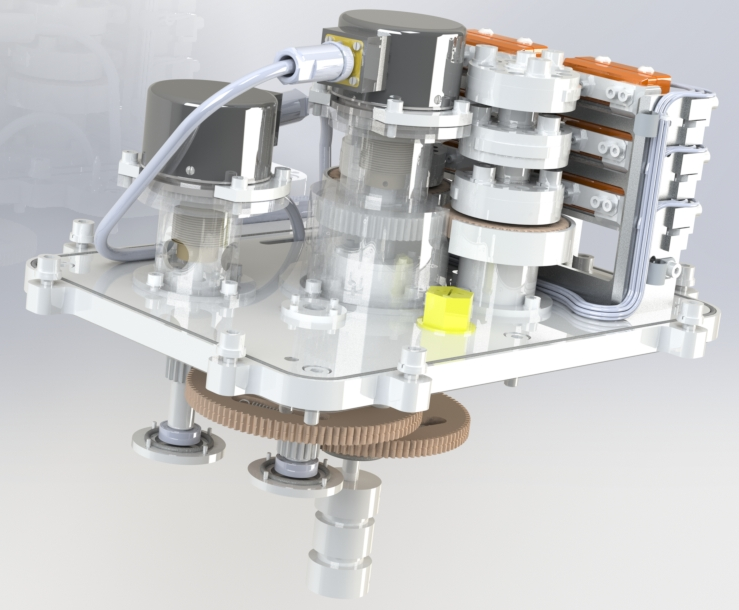
\includegraphics[width=0.6\textwidth]{Reductor.png}
    \caption{Редуктор УМ}
    \label{Reductor}
  \end{figure}


\begin{figure}[!h]
    \centering
    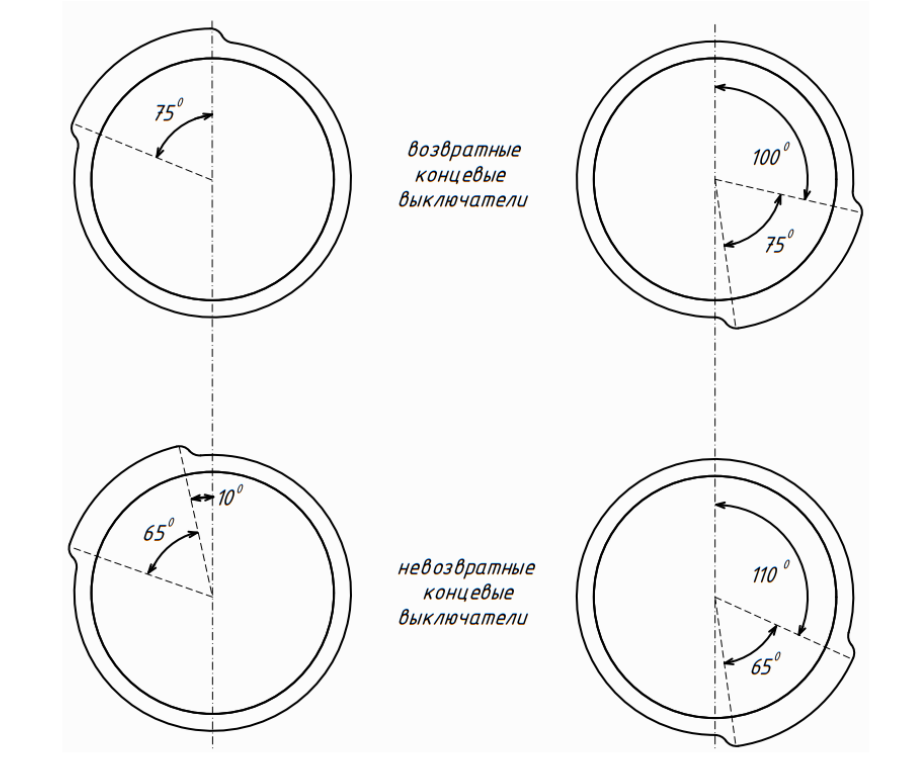
\includegraphics[width=0.8\textwidth]{Эскиз_профилей_кулачков.png} 
    \caption{Эскиз профилей кулачков УМ}
    \label{cams}
\end{figure}

\begin{figure}[h]
    \centering
    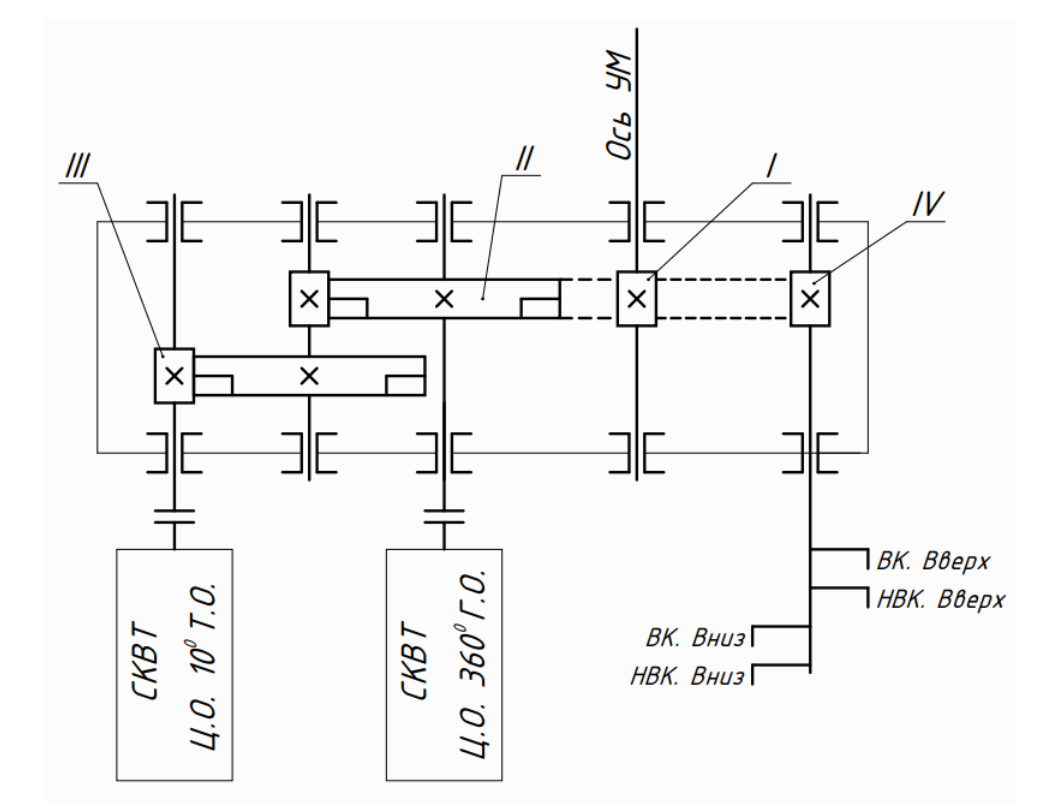
\includegraphics[width=150mm]{Кинематическая_схема_редуктора.png}
    \caption{Кинематическая схема редуктора}
    \label{kinematic}
  \end{figure}

\subsubsection{Особенности конструкции}
\begin{itemize}
    \item \textbf{Доступность обслуживания}: Конструкция редуктора предусматривает удобный доступ к датчикам и выключателям как на этапе заводской сборки, так и во время эксплуатационного обслуживания.
    \item \textbf{Защита от перегрузок}: Невозвратные выключатели исключают риск повреждения антенны при выходе за пределы рабочих углов.
\end{itemize}




Таком образом, в конструкцию приборного редуктора УМ заложено сочетание высокой точности измерений (благодаря двухотсчетной схеме)
и надежная защиту от аварийных ситуаций. Использование стандартизированных компонентов обеспечивает ремонтопригодность и адаптивность системы.


\newpage
\section{Определение погрешностей многоступенчатого передаточного механизма}
Далее нужно определить ошибку, вносимую механизмом редуктора.

Согласно \cite{Kin}, погрешность каждой передачи приводится к выходному $n$-му звену, будучи поделена на передаточное отношение от данной передачи до выходного звена. 
При наличии паразитных звеньев их следует учитывать дважды -- как ведомое в паре с предыдущим и ведущее в паре с последующим звеном кинематической цепи.

\subsection{Максимальная кинематическая погрешность $\delta\phi_{\Sigma \text{max}}$ и максимальный кинематический мертвый ход $j\phi_{\Sigma \text{max}}$}

\begin{equation}
    \delta\phi_{\Sigma \text{max}} = \delta\phi_{\text{max}12} + \delta\phi_{\text{max}34} + \dots + \delta\phi_{\text{max}(n-1)n}, \quad y \geq \pi. \quad \text{МКХ.} \tag{6.53}
\end{equation}

\begin{equation}
    j\phi_{\Sigma \text{max}} = \frac{j_{\text{max}12} + j_{\text{max}34} + \dots + j_{\text{max}(n-1)n}}{i_m}, \quad y \geq \pi. \quad \text{МКХ.} \tag{6.54}
\end{equation}

где $n$ -- номер выходного колеса $z_n$.

\subsection{Минимальная кинематическая погрешность $\delta\phi_{\Sigma \text{min}}$ и минимальный кинематический мертвый ход $j\phi_{\Sigma \text{min}}$}

\begin{equation}
    \delta\phi_{\Sigma \text{min}} = \delta\phi_{\text{min}12} + \delta\phi_{\text{min}34} + \dots + \delta\phi_{\text{min}(n-1)n}, \quad y \geq \pi. \quad \text{МКХ.} \tag{6.55}
\end{equation}

\begin{equation}
    j\phi_{\Sigma \text{min}} = \frac{j_{\text{min}12} + j_{\text{min}34} + \dots + j_{\text{min}(n-1)n}}{i_m}, \quad y \geq \pi. \quad \text{МКХ.} \tag{6.56}
\end{equation}




\section{Расчет кинематики проектного редуктора}
\subsection{Методика расчета кинематической погрешности}

Кинематическая погрешность редуктора определяется как отклонение угла поворота выходного вала от теоретически заданного значения. 
Для её расчета используется метод, основанный на ГОСТ 21098 и ГОСТ 1643, учитывающий погрешности изготовления зубчатых передач. Основные этапы расчета включают:
\begin{itemize}
    \item Определение кинематической погрешности каждой ступени редуктора.
    \item Преобразование линейных погрешностей в угловые единицы.
    \item Суммирование погрешностей с учетом передаточных отношений.
\end{itemize}

\subsubsection{Формулы расчета}
\begin{itemize}
    \item Минимальная кинематическая погрешность ступени:
        \[
        F'_{i0_{\text{min}}} = 0.62 \cdot K_S \cdot (F'_{i1} + F'_{i2}),
        \]
        где \( F'_i = F_p + f_f \) — погрешность колеса, \( K_S \) — коэффициент фазовой компенсации.
    \item Перевод в угловые минуты:
        \[
        \Delta\phi_{i0} = \frac{6.88 \cdot F'_{i0}}{d},
        \]
        где \( d \) — делительный диаметр ведомого колеса.
    \item Суммарная погрешность механизма:
        \[
        \Delta\phi_{\sum} = \frac{\Delta\phi_{12}}{i_{34}} + \Delta\phi_{34}.
        \]
\end{itemize}

% \subsection{Анализ вариантов кинематических схем}
% \subsubsection*{Вариант 1}
% \begin{itemize}
%     \item \textbf{Параметры шестерен:} 
%         \begin{tabular}{|c|c|c|c|c|}
%             \hline
%             Колесо & Число зубьев & \( F_p \), мкм & \( f_f \), мкм & \( K_S \) \\ \hline
%             1 & 102 & 45 & 8 & 0.74 \\ \hline
%             2 & 34 & 25 & 8 & — \\ \hline
%         \end{tabular}
%     \item \textbf{Расчет:}
%         \[
%         F'_{i0_{\text{min12}}} = 0.62 \cdot 0.74 \cdot (45 + 8 + 25 + 8) = 39.25 \, \text{мкм}.
%         \]
%         \[
%         \Delta\phi_{12} = \frac{6.88 \cdot 39.25}{34} = 7.941'.
%         \]
%     \item \textbf{Итог:} Суммарная погрешность механизма:
%         \[
%         \Delta\phi_{\sum} = \frac{7.941}{0.33} + 7.941 = 32.01'.
%         \]
% \end{itemize}

% \subsubsection*{Вариант 2}
% \begin{itemize}
%     \item \textbf{Параметры шестерен:} 
%         \begin{tabular}{|c|c|c|c|c|}
%             \hline
%             Колесо & Число зубьев & \( F_p \), мкм & \( f_f \), мкм & \( K_S \) \\ \hline
%             1 & 100 & 32 & 8 & 0.76 \\ \hline
%             3 & 102 & 45 & 8 & 0.88 \\ \hline
%         \end{tabular}
%     \item \textbf{Расчет:}
%         \[
%         F'_{i0_{\text{min34}}} = 0.62 \cdot 0.88 \cdot (45 + 8 + 20 + 8) = 44.19 \, \text{мкм}.
%         \]
%         \[
%         \Delta\phi_{34} = \frac{6.88 \cdot 44.19}{17} = 17.88'.
%         \]
%     \item \textbf{Итог:} Суммарная погрешность:
%         \[
%         \Delta\phi_{\sum} = \frac{4.61}{0.17} + 17.88 = 45.00'.
%         \]
% \end{itemize}

% \subsubsection*{Вариант 3}
% \begin{itemize}
%     \item \textbf{Особенность:} Упрощенная схема с двумя шестернями.
%     \item \textbf{Параметры:}
%         \begin{tabular}{|c|c|c|c|c|}
%             \hline
%             Колесо & Число зубьев & \( F_p \), мкм & \( f_f \), мкм & \( K_S \) \\ \hline
%             1 & 138 & 45 & 8 & 0.98 \\ \hline
%         \end{tabular}
%     \item \textbf{Итог:} 
%         \[
%         \Delta\phi_{1-2} = \frac{2.642}{0.12} + 11.332 = 33.35'.
%         \]
% \end{itemize}

\subsection{Расчет стенда рис. \ref{kinematic}}
\begin{itemize}
    \item \textbf{Параметры:}
        \begin{tabular}{|c|c|c|c|c|}
            \hline
            Колесо & Число зубьев & \( F_p \), мкм & \( f_f \), мкм & \( K_S \) \\ \hline
            1 & 17 & 20 & 8 & 0.98 \\ \hline
        \end{tabular}
%     \item \textbf{Итог:}
%         \[
%         \Delta\phi_{\sum} = \frac{19.92}{6} + 19.92 = 23.24'.
%         \]
\end{itemize}
% Таким образом стенд показывает погрешность \(23.24'\), что подтверждает адекватность методики расчета.


\noindent Расчет для первой пары колес (1 и 2):
\begin{align*}
F'_{i0min1} &= 0.62 \cdot 0.98 \cdot ((45 + 8) + (20 + 8)) \\
&= 0.62 \cdot 0.98 \cdot 81 = 49,\!2156\ \text{мкм}
\end{align*}

\noindent Расчет для второй пары колес (3 и 4):
\begin{align*}
F'_{i0min2} &= 0.62 \cdot 0.98 \cdot ((45 + 8) + (20 + 8)) \\
&= 0.62 \cdot 0.98 \cdot 81 = 49,\!2156\ \text{мкм}
\end{align*}

Угловые погрешности зацеплений:
\begin{align*}
\Delta \phi_{12} &= \frac{6.88 \cdot 49.216}{17} = 19,\!92' \\
\Delta \phi_{34} &= \frac{6.88 \cdot 49.216}{17} = 19,\!92'
\end{align*}

Кинематическая погрешность механизма, приведенная к выходному звену:
\begin{equation}
\Delta \phi_{\sum} = \frac{\Delta \phi_{12}}{i_{34}} + \Delta \phi_{34}
\end{equation}

\noindent При передаточном отношении $i_{34} = 6$:
\begin{align*}
\Delta \phi_{\sum} &= \frac{19.92}{6} + 19.92 \\
&= 3.32 + 19.92 = 23,\!24'
\end{align*}

Таким образом, расчетная минимальная кинематическая погрешность стенда составляет 23,\!24 угловых минуты.





